{
\renewcommand{\thechapter}{\arabic{chapter}N}
\setcounter{chapter}{15}
\exam{Exam normal 2015/16}

\question{Question 1}
Assume you are managing the process of placing outdoor billboards in a part of the A1 highway (north-south direction) with $N$ kilometers. Vector \texttt{pos[]} specifies possible places for billboards, where \texttt{pos[i]} is the distance in $\SI{}{\kilo\metre}$ from point $i$ to the end of the road (assume this vector to be sorted in increasing order). On placing a billboard, a value is charged which depends on the place the billboard is placed. Consider \texttt{value[]} to be the vector representing values to be charged, where \texttt{value[i]} is the value to be charged for placing a billboard at position \texttt{pos[i]}. You cannot place billboards less than $\SI{5}{\kilo\metre}$ appart. You want to find the maximum value that can be charged for billboards.

\questionitem{Item a}
Implement (in C++ or pseudocode) a solution for this problem, using a greedy algorithm. Mention its time complexity. Is that algorithm optimal? Explain.

\ansseparator

\lstinputlisting[language=C++]{2016N_01a.cpp}

This algorithm runs in time $O(N)$, since it iterates once over each of the $N$ potential billboard places.

This algorithm works by selecting the billboard with smallest \texttt{pos} that complies with the $\SI{5}{\kilo\metre}$ rule.

This algorithm is not optimal. To prove that, we will present a test case for which our algorithm produces a sub-optimal solution: $pos = \langle 1, 2 \rangle$, $value = \langle 1, 10 \rangle$. Our algorithm would only choose to place a billboard at 0 (with profit 1), but the solution of placing a billboard at 1 (with profit 10) is better, thus our algorithm has not found the optimal solution, otherwise it would be impossible to mention a better solution.

\questionitem{Item b}
Formalize a solution to this problem using dynamic programming. Implement (in C++ or pseudocode) that solution and mention its time complexity. Explain.\\

\textbf{Suggestion:} if you wish, you may consider a value \texttt{e[j]} as being the closest place from \texttt{pos[j]} whose distance to \texttt{j} is greater than or equal to $\SI{5}{\kilo\metre}$.

\ansseparator

A state is uniquely represented by:
\begin{itemize}
    \item $i$, the place we are about to process.
    \item $d$, the location from which we can install the next billboard.
\end{itemize}

$S_i^d$ is the profit we make in state $(i,d)$.

The base case is $S_0^0 = 0$, meaning we have not yet installed any billboards and are deciding to install a billboard or not in the first place.

Each state $(i,d)$ can contribute to two more states:
\begin{itemize}
    \item If a billboard can be placed ($d \leq pos[i]$) then $S_{i+1}^{pos[i]+5-1}$ can be $S_i^d + value[i]$.
    \item $S_{i+1}^d = S_i^d$ if we do not place a billboard at $i$.
\end{itemize}

The solution is $\max_{d \in \mathbb{R}}\{S_{N}^d\}$.

\newpage
\lstinputlisting[language=C++]{2016N_01b.cpp}

\question{Question 2}
The following directed graph represents a map, where vertices are cities and the value of an edge is the distance between adjacent cities. Mr Joaquim lives in city $A$ and intends to visit his family in city $G$.

\begin{center}
    \begin{tikzpicture}[->,>=stealth',node distance=1.61cm,initial text=$ $,]
        \small
		\node[state](A) {$A$};
        \node[state, above of=A](B) {$B$};
        \node[state, above of=B](C) {$C$};
        \node[state, left  of=A](E) {$E$};
        \node[state, above of=E](D) {$D$};
        \node[state, above of=D](G) {$G$};
        \node[state, left  of=D](F) {$F$};
        
        \draw   (A) 	edge[bend right=40, right] node{8} (C)
                (A) 	edge[above] node{7} (E)
                (B) 	edge[right] node{2} (A)
                (B) 	edge[bend left=10, below] node{3} (D)
                (C) 	edge[right] node{4} (B)
                (C) 	edge[above] node{1} (D)
                (D) 	edge[bend left=10, above] node{1} (B)
                (D) 	edge[above] node{4} (F)
                (D) 	edge[left ] node{9} (G)
                (E) 	edge[right] node{3} (D)
                (E) 	edge[bend right=10, above] node{10} (F)
                (F) 	edge[bend right=10, below] node{9} (E)
                (F) 	edge[left ] node{3} (G)
                (G) 	edge[above] node{6} (C)
                
                ;
	\end{tikzpicture}
\end{center}

\questionitem{Item a}
Find the path that Mr Joaquin should follow to travel the least distance. Explain.

\ansseparator

We will find the shortest path from $A$ to $G$ using Dijkstra's algorithm. The following table is a trace for Dijkstra's algorithm.

\begin{algorithm}[H]
    \caption{Dijkstra's algorithm}
    \begin{algorithmic}[1]
        \Function{Dijkstra}{$G(V,E)$, $s$}
            \For{$v \in V$}{ $dist(v) \gets \infty,~prev(v) \gets \text{NULL}$}
            \EndFor
            \State {$Q \gets V$}
            \State {$dist(s) \gets 0$}
            \While{$|Q| > 0$}
                \State {$u \gets \text{vertex of $Q$ with least $dist(u)$}$}
                \State {$Q \gets Q \backslash \{u\}$}
                \For{$v \in \Call{Adj}{G, u}$}
                    \State{$c' \gets dist(u) + w(u,v)$}
                    \If{$c' < dist(v)$}
                        \State{$dist(v) \gets c',~prev(v) \gets u$}
                    \EndIf
                \EndFor
            \EndWhile
            \State \Return $dist$, $prev$
        \EndFunction
    \end{algorithmic}
\end{algorithm}

\begin{center} \begin{tabular}{r | c c c}
    \textbf{Line} & $(dist, prev)$                                                                                              & $Q$                 & $u$ \\ \hline
    3             & $\langle (\infty, -), (\infty, -), (\infty, -), (\infty, -), (\infty, -), (\infty, -), (\infty, -) \rangle$ & $\{A,B,C,D,E,F,G\}$ & -   \\
    5             & $\langle (     0, -), (\infty, -), (\infty, -), (\infty, -), (\infty, -), (\infty, -), (\infty, -) \rangle$ & $\{A,B,C,D,E,F,G\}$ & -   \\
    8             & $\langle (     0, -), (\infty, -), (\infty, -), (\infty, -), (\infty, -), (\infty, -), (\infty, -) \rangle$ & $\{  B,C,D,E,F,G\}$ & $A$ \\
    5             & $\langle (     0, -), (\infty, -), (     8, A), (\infty, -), (     7, A), (\infty, -), (\infty, -) \rangle$ & $\{  B,C,D,E,F,G\}$ & $A$ \\
    8             & $\langle (     0, -), (\infty, -), (     8, A), (\infty, -), (     7, A), (\infty, -), (\infty, -) \rangle$ & $\{  B,C,D,  F,G\}$ & $E$ \\
    5             & $\langle (     0, -), (\infty, -), (     8, A), (    10, E), (     7, A), (    17, E), (\infty, -) \rangle$ & $\{  B,C,D,  F,G\}$ & $E$ \\
    8             & $\langle (     0, -), (\infty, -), (     8, A), (    10, E), (     7, A), (    17, E), (\infty, -) \rangle$ & $\{  B,  D,  F,G\}$ & $C$ \\
    5             & $\langle (     0, -), (    12, C), (     8, A), (     9, C), (     7, A), (    17, E), (\infty, -) \rangle$ & $\{  B,  D,  F,G\}$ & $C$ \\
    8             & $\langle (     0, -), (    12, C), (     8, A), (     9, C), (     7, A), (    17, E), (\infty, -) \rangle$ & $\{  B,      F,G\}$ & $D$ \\
    5             & $\langle (     0, -), (    10, D), (     8, A), (     9, C), (     7, A), (    13, D), (    18, D) \rangle$ & $\{  B,      F,G\}$ & $D$ \\
    8             & $\langle (     0, -), (    10, D), (     8, A), (     9, C), (     7, A), (    13, D), (    18, D) \rangle$ & $\{          F,G\}$ & $B$ \\
    5             & $\langle (     0, -), (    10, D), (     8, A), (     9, C), (     7, A), (    13, D), (    18, D) \rangle$ & $\{          F,G\}$ & $B$ \\
    8             & $\langle (     0, -), (    10, D), (     8, A), (     9, C), (     7, A), (    13, D), (    18, D) \rangle$ & $\{            G\}$ & $F$ \\
    5             & $\langle (     0, -), (    10, D), (     8, A), (     9, C), (     7, A), (    13, D), (    16, F) \rangle$ & $\{            G\}$ & $F$ \\
    8             & $\langle (     0, -), (    10, D), (     8, A), (     9, C), (     7, A), (    13, D), (    16, F) \rangle$ & $\{             \}$ & $G$ \\
    5             & $\langle (     0, -), (    10, D), (     8, A), (     9, C), (     7, A), (    13, D), (    16, F) \rangle$ & $\{             \}$ & $G$ \\
    12            & $\langle (     0, -), (    10, D), (     8, A), (     9, C), (     7, A), (    13, D), (    16, F) \rangle$ & $\{             \}$ & -   \\
\end{tabular} \end{center}

The shortest path from $A$ to $G$ is $A \rightarrow C \rightarrow D \rightarrow F \rightarrow G$, with a total weight of 16.

\questionitem{Item b}
Mr Joaquim is now worried with the travel's cost. His car consumes $\SI{1}{\litre}$ per unit distance. The price of gasoline in cities $\{A,B,C,D,E,F,G\}$ is $\{1\eqeuro, 2\eqeuro, 1\eqeuro, 2\eqeuro, 1\eqeuro, 1\eqeuro, 1\eqeuro\}$ respectively. Mr Joaquim only fills when needed (when he does not have enough gasoline to cross the road he wants to cross) and always fills $\SI{10}{\litre}$ of gasoline. Initially the car tank is empty. Implement an algorithm (in C++ or pseudocode) to determine the path Mr Joaquim should use so as to minimize the money spent on gasoline, and show the path he should follow. Explain. Suggestion: change Dijkstra's algorithm.

\ansseparator

\begin{algorithm}[H]
    \caption{Dijkstra's algorithm}
    \begin{algorithmic}[1]
        \Function{Dijkstra}{$G(V,E,w)$, $price$, $s$, $d$}
            \For{$v \in V$}{ $cost(v) \gets \infty,~prev(v) \gets \text{NULL},~tank(v) \gets 0$}
            \EndFor
            \State {$Q \gets V$}
            \State {$cost(s) \gets 0$}
            \While{$|Q| > 0$}
                \State {$u \gets \text{vertex of $Q$ with least $dist(u)$}$}
                \State {$Q \gets Q \backslash \{u\}$}
                \If{$u = d$}{ break}
                \EndIf
                \For{$v \in \Call{Adj}{G, u}$}
                    \State{$c' \gets cost(u) + (w(u,v) \leq tank(u) ? 0 : 10*price(u))$}
                    \State{$t' \gets tank(u) + (w(u,v) \leq tank(u) ? 0 : 10) - w(u,v) $}
                    \If{$c' < cost(v)\text{ \textbf{or} }(c' = cost(v) \text{ \textbf{and} } t' > tank(v))$}
                        \State{$cost(v) \gets c',~prev(v) \gets u,~tank(v) \gets t'$}
                    \EndIf
                \EndFor
            \EndWhile
            \State \Return $dist$, $prev$
        \EndFunction
    \end{algorithmic}
\end{algorithm}

\begin{center}
    \begin{tikzpicture}[->,>=stealth',node distance=3cm,initial text=$ $,]
        \small
		\node[state            , fill=visitedcolor](A) {$A (     0, -, 0)$};
        \node[state, above of=A, fill=visitedcolor](B) {$B (    10, D, 0)$};
        \node[state, above of=B, fill=visitedcolor](C) {$C (    10, A, 2)$};
        \node[state, left  of=A, fill=visitedcolor](E) {$E (    10, A, 3)$};
        \node[state, above of=E, fill=visitedcolor](D) {$D (    10, C, 1)$};
        \node[state, above of=D, fill=visitedcolor](G) {$G (    20, F, 0)$};
        \node[state, left  of=D, fill=visitedcolor](F) {$F (    20, E, 3)$};
        
        \draw   (A) 	edge[bend right=40, right] node{8} (C)
                (A) 	edge[above] node{7} (E)
                (B) 	edge[right] node{2} (A)
                (B) 	edge[bend left=10, below] node{3} (D)
                (C) 	edge[right] node{4} (B)
                (C) 	edge[above] node{1} (D)
                (D) 	edge[bend left=10, above] node{1} (B)
                (D) 	edge[above] node{4} (F)
                (D) 	edge[left ] node{9} (G)
                (E) 	edge[right] node{3} (D)
                (E) 	edge[bend right=10, above] node{10} (F)
                (F) 	edge[bend right=10, below] node{9} (E)
                (F) 	edge[left ] node{3} (G)
                (G) 	edge[above] node{6} (C)
                
                ;
	\end{tikzpicture}
\end{center}

I am almost absolutely sure this algorithm is not optimal in these conditions, although I am not sure why it is not optimal.

The best path is $A \rightarrow E \rightarrow F \rightarrow G$. Mr Joaquim must refill his tank in $A$ and $E$ so he spends 20\euro.

\questionitem{Item c}
Mr Joaquim now wants to know/travel through all roads, but he does not want to go through any of them more than once. Is that possible? If so, show the path he should follow.

\ansseparator

\begin{center}
    \begin{tikzpicture}[->,>=stealth',node distance=2cm,initial text=$ $,]
		\node[state            , fill=gray!50 ](A) {$A$};
        \node[state, above of=A](B) {$B$};
        \node[state, above of=B](C) {$C$};
        \node[state, left  of=A](E) {$E$};
        \node[state, above of=E](D) {$D$};
        \node[state, above of=D, fill=gray!100](G) {$G$};
        \node[state, left  of=D](F) {$F$};
        
        \draw   (A) 	edge[bend right=40, right] node{8} (C)
                (A) 	edge[above] node{7} (E)
                (B) 	edge[right] node{2} (A)
                (B) 	edge[bend left=10, below] node{3} (D)
                (C) 	edge[right] node{4} (B)
                (C) 	edge[above] node{1} (D)
                (D) 	edge[bend left=10, above] node{1} (B)
                (D) 	edge[above] node{4} (F)
                (D) 	edge[left ] node{9} (G)
                (E) 	edge[right] node{3} (D)
                (E) 	edge[bend right=10, above] node{10} (F)
                (F) 	edge[bend right=10, below] node{9} (E)
                (F) 	edge[left ] node{3} (G)
                (G) 	edge[above] node{6} (C)
                
                ;
	\end{tikzpicture}
\end{center}

In white are vertices with in-degree equal to out-degree. In light gray are vertices with out-degree larger than in-degree by 1. In dark gray are vertices with in-degree larger than out-degree by 1. This means there is not an eulerian cycle because not all vertices have in-degree equal to out-degree, but there is an eulerian path starting in $A$ and ending in $G$, which can be $A \rightarrow E \rightarrow F \rightarrow E \rightarrow D \rightarrow B \rightarrow A \rightarrow C \rightarrow B \rightarrow D \rightarrow F \rightarrow G \rightarrow C \rightarrow D \rightarrow G$.

\question{Question 3}
Consider the following undirected weighted graph $G$, where vertices represent places and an edge's value represents the cost associated to the connection between adjacent places.

\begin{center}
    \begin{tikzpicture}[-,>=stealth',node distance=2cm,initial text=$ $,]
		\node[state            ](A) {$A$};
        \node[state, right of=A](B) {$B$};
        \node[state, right of=B](C) {$C$};
        \node[state, right of=C](D) {$D$};
        \node[state, right of=D](E) {$E$};
        
        \node[state, below of=A](F) {$F$};
        \node[state, right of=F](G) {$G$};
        \node[state, right of=G](H) {$H$};
        \node[state, right of=H](I) {$I$};
        
        \node[state, below of=F](J) {$J$};
        \node[state, right of=J](K) {$K$};
        \node[state, right of=K](L) {$L$};
        \node[state, right of=L](M) {$M$};
        

        \draw   (A) 	edge[above] node{ 2} (B)
                (B) 	edge[above] node{13} (C)
                (C) 	edge[above] node{ 2} (D)
                (D) 	edge[above] node{ 1} (E)
                (A) 	edge[left ] node{ 5} (F)
                (A) 	edge[left ] node{ 2} (G)
                (B) 	edge[left ] node{ 8} (G)
                (C) 	edge[left ] node{ 5} (H)
                (D) 	edge[left ] node{ 2} (H)
                (D) 	edge[left ] node{ 7} (I)
                (E) 	edge[left ] node{12} (I)
                (E) 	edge[right] node{ 6} (M)
                (F) 	edge[left ] node{ 4} (J)
                (G) 	edge[left ] node{ 2} (J)
                (G) 	edge[left ] node{ 1} (K)
                (H) 	edge[left ] node{ 3} (K)
                (H) 	edge[left ] node{ 4} (L)
                (I) 	edge[left ] node{ 1} (L)
                (I) 	edge[left ] node{ 2} (M)
                (J) 	edge[below] node{ 4} (K)
                (K) 	edge[below] node{ 7} (L)
                (L) 	edge[below] node{ 3} (M)
                ;
	\end{tikzpicture}
\end{center}

\questionitem{Item a}
Find a minimum spanning tree, using the algorithm you find convenient. Present the order in which vertices are added to the minimum spanning tree, according to the algorithm you chose. Explain.

\ansseparator

I will use Kruskal's algorithm. This algorithm consists of initially representing a graph as a forest of individual nodes; we order all edges by weight and process them by increasing weight, selecting edges that connect two separate trees until there is only one tree.

We will sort edges by increasing weight, then increasing first node and then increasing second node.

\begin{center}
    \begin{tikzpicture}[-,>=stealth',node distance=2cm,initial text=$ $,]
        \small
		\node[state            ](A) {$A$};
        \node[state, right of=A](B) {$B$};
        \node[state, right of=B](C) {$C$};
        \node[state, right of=C](D) {$D$};
        \node[state, right of=D](E) {$E$};
        
        \node[state, below of=A](F) {$F$};
        \node[state, right of=F](G) {$G$};
        \node[state, right of=G](H) {$H$};
        \node[state, right of=H](I) {$I$};
        
        \node[state, below of=F](J) {$J$};
        \node[state, right of=J](K) {$K$};
        \node[state, right of=K](L) {$L$};
        \node[state, right of=L](M) {$M$};
        

        \draw   (A) 	edge[above, line width=1.5pt] node{ 2} (B)
                (B) 	edge[above] node{13} (C)
                (C) 	edge[above, line width=1.5pt] node{ 2} (D)
                (D) 	edge[above, line width=1.5pt] node{ 1} (E)
                (A) 	edge[left ] node{ 5} (F)
                (A) 	edge[left , line width=1.5pt] node{ 2} (G)
                (B) 	edge[left ] node{ 8} (G)
                (C) 	edge[left ] node{ 5} (H)
                (D) 	edge[left , line width=1.5pt] node{ 2} (H)
                (D) 	edge[left ] node{ 7} (I)
                (E) 	edge[left ] node{12} (I)
                (E) 	edge[right] node{ 6} (M)
                (F) 	edge[left , line width=1.5pt] node{ 4} (J)
                (G) 	edge[left , line width=1.5pt] node{ 2} (J)
                (G) 	edge[left , line width=1.5pt] node{ 1} (K)
                (H) 	edge[left , line width=1.5pt] node{ 3} (K)
                (H) 	edge[left , line width=1.5pt] node{ 4} (L)
                (I) 	edge[left , line width=1.5pt] node{ 1} (L)
                (I) 	edge[left , line width=1.5pt] node{ 2} (M)
                (J) 	edge[below] node{ 4} (K)
                (K) 	edge[below] node{ 7} (L)
                (L) 	edge[below] node{ 3} (M)
                ;
	\end{tikzpicture}
\end{center}

\begin{center} \begin{tabular}{l | r c}
    \textbf{Edge}    & \textbf{Weight} & \textbf{Action} \\ \hline
    $D \text{---} E$ &               1 & Added \\
    $G \text{---} K$ &               1 & Added \\
    $I \text{---} L$ &               1 & Added \\
    $A \text{---} B$ &               2 & Added \\
    $A \text{---} G$ &               2 & Added \\
    $C \text{---} D$ &               2 & Added \\
    $D \text{---} H$ &               2 & Added \\
    $G \text{---} J$ &               2 & Added \\
    $I \text{---} M$ &               2 & Added \\
    $H \text{---} K$ &               3 & Added \\
    $L \text{---} M$ &               3 & Ignored \\
    $F \text{---} J$ &               4 & Added \\
    $H \text{---} L$ &               4 & Added \\
    $J \text{---} K$ &               4 & Ignored \\
    $A \text{---} F$ &               5 & Ignored \\
    $C \text{---} H$ &               5 & Ignored \\
    $E \text{---} M$ &               6 & Ignored \\
    $D \text{---} I$ &               7 & Ignored \\
    $K \text{---} L$ &               7 & Ignored \\
    $B \text{---} G$ &               8 & Ignored \\
    $E \text{---} I$ &              12 & Ignored \\
    $B \text{---} C$ &              13 & Ignored
\end{tabular} \end{center}

Edges were added by the following order: $D \text{---} E$, $G \text{---} K$, $I \text{---} L$, $A \text{---} B$, $A \text{---} G$, $C \text{---} D$, $D \text{---} H$, $G \text{---} J$, $I \text{---} M$, $H \text{---} K$, $F \text{---} J$, $H \text{---} L$.

\questionitem{Item b}
Implement an efficient algorithm (in pseudocode) that, knowing the minimum spanning tree $T$ of a graph $G$, identifies the second minimum spanning tree ($T_2$). $T_2$ is the spanning tree of $G$ having the least cost, other than $T$. Note that $T$ and $T_2$ differ only by one edge.

\ansseparator

\begin{algorithm}[H]
    \caption{Second MST}
    \begin{algorithmic}[1]
        \Function{SecondMST}{$G(V,E,w)$, $MST$}
            \State{$res \gets \text{NULL},~c \gets \infty$}
            \For{$(u,v) \in MST$}
                \State{$MST' \gets MST \backslash (u,v)$}
                \State{$G' \gets (V, MST', w)$} \Comment{Has two tree components}
                \State{$W' \gets \sum_{(u',v') \in MST'}{w(u',v')}$} \Comment{Sum of all weights in $G'$}
                \State{$S_1 \gets \Call{DFS}{G', u}$} \Comment{Tree component containing $u$}
                \State{$S_2 \gets \Call{DFS}{G', v}$} \Comment{Tree component containing $v$}
                \For{$(u',v') \in E$}
                    \If{$u' \in S_1 \textbf{ and } v' \in S_2 \textbf{ and } W'+w(u',v') < c$}
                        \State{$res \gets MST' \cup \{(u',v')\},~c \gets W'+w(u',v')$}
                    \EndIf
                \EndFor
            \EndFor
            \State \Return $res$
        \EndFunction
    \end{algorithmic}
\end{algorithm}

\question{Question 3}
A drainage system was designed, according to the following graph, to transport 50,000 units of volume (uv) of waste water from the source in node $E$ to the sink in node $C$. Transport is made by gravity, meaning canals have no pressure; in the network the canals' inclination is indicated with the direction of the arows, and their capacities in parenthesis are given in 1,000 uv. Answer the following questions, presenting the proper justification.

\begin{center}
    \begin{tikzpicture}[->,>=stealth',node distance=2cm,initial text=$ $,]
		\node[state            ](A) {$A$};
        \node[state, below right of=A](D) {$D$};
        \node[state, above right of=D](B) {$B$};
        \node[state, right of=B](C) {$C$};
        \node[state, below right of=D](G) {$G$};
        \node[state, below left  of=D](F) {$F$};
        \node[state, left  of=F](E) {$E$};

        \draw   (A) 	edge[above] node{50} (B)
                (A) 	edge[above] node{20} (D)
                (B) 	edge[above] node{50} (C)
                (B) 	edge[right] node{10} (G)
                (D) 	edge[above] node{ 5} (B)
                (D) 	edge[above] node{ 5} (F)
                (E) 	edge[above] node{50} (F)
                (F) 	edge[left ] node{10} (A)
                (G) 	edge[left ] node{20} (D)
                (G) 	edge[below] node{50} (F)
                ;
	\end{tikzpicture}
\end{center}

\questionitem{Item a}
Can the network transport the desired volume of 50,000 uv? What is the maximum flow this network can transport?

\ansseparator

We will use Edmonds-Karp algorithm to find the maximum flow from $E$ to $C$. This algorithm operates by finding the shortest augmenting path in the residues graph and augment flow through that path, until there are no more augmenting paths. It specializes the Ford-Fulkerson algorithm by choosing the \textbf{shortest} (not \emph{any}) augmenting path.

Below is the algorithm trace, in the form of the residues graph.

\begin{center} \begin{tabular}{c | c}
    \begin{tikzpicture}[->,>=stealth',node distance=1.74cm,initial text=$ $,]
        \small
        \node[state            ](A) {$A$};
        \node[state, below right of=A](D) {$D$};
        \node[state, above right of=D](B) {$B$};
        \node[state, right of=B, accepting](C) {$C$};
        \node[state, below right of=D](G) {$G$};
        \node[state, below left  of=D](F) {$F$};
        \node[state, left  of=F, initial](E) {$E$};

        \draw   (A) 	edge[above, line width=1.5pt] node{50} (B)
                (A) 	edge[above] node{20} (D)
                (B) 	edge[above, line width=1.5pt] node{50} (C)
                (B) 	edge[right] node{10} (G)
                (D) 	edge[above] node{ 5} (B)
                (D) 	edge[above] node{ 5} (F)
                (E) 	edge[above, line width=1.5pt] node{50} (F)
                (F) 	edge[left , line width=1.5pt] node{10} (A)
                (G) 	edge[left ] node{20} (D)
                (G) 	edge[below] node{50} (F)
                ;
    \end{tikzpicture} &
    \begin{tikzpicture}[->,>=stealth',node distance=1.74cm,initial text=$ $,]
        \small
        \node[state            ](A) {$A$};
        \node[state, below right of=A](D) {$D$};
        \node[state, above right of=D](B) {$B$};
        \node[state, right of=B, accepting](C) {$C$};
        \node[state, below right of=D](G) {$G$};
        \node[state, below left  of=D](F) {$F$};
        \node[state, left  of=F, initial](E) {$E$};

        \draw   (A) 	edge[bend right=10, below] node{40} (B)
                (B) 	edge[bend right=10, above] node{10} (A)
                (A) 	edge[above] node{20} (D)
                (B) 	edge[bend right=10, below] node{40} (C)
                (C) 	edge[bend right=10, above] node{10} (B)
                (B) 	edge[right] node{10} (G)
                (D) 	edge[above] node{ 5} (B)
                (D) 	edge[above] node{ 5} (F)
                (E) 	edge[bend right=10, below] node{40} (F)
                (F) 	edge[bend right=10, above] node{10} (E)
                (F) 	edge[bend right=10, right, dashed] node{0} (A)
                (A) 	edge[bend right=10, left ] node{10} (F)
                (G) 	edge[left ] node{20} (D)
                (G) 	edge[below] node{50} (F)
                ;
    \end{tikzpicture} \\
    &
    Total flow: 10
\end{tabular} \end{center}

The maximum flow from $E$ to $C$ is thus 10,000 uv, so the network cannot transport the desired volume of 50,000 uv.

\questionitem{Item b}
What happens to the maximum volume if a new sink, additionally to $C$, is placed in $D$?

\ansseparator

\begin{center} \begin{tabular}{c | c}
    \begin{tikzpicture}[->,>=stealth',node distance=1.74cm,initial text=$ $,]
        \small
        \node[state            ](A) {$A$};
        \node[state, below right of=A](D) {$D$};
        \node[state, above right of=D](B) {$B$};
        \node[state, right of=B, accepting](C) {$C$};
        \node[state, below right of=D](G) {$G$};
        \node[state, below left  of=D](F) {$F$};
        \node[state, left  of=F, initial](E) {$E$};

        \draw   (A) 	edge[above, line width=1.5pt] node{50} (B)
                (A) 	edge[above] node{20} (D)
                (B) 	edge[above, line width=1.5pt] node{50} (C)
                (B) 	edge[right] node{10} (G)
                (D) 	edge[above] node{ 5} (B)
                (D) 	edge[below] node{50} (C)
                (D) 	edge[above] node{ 5} (F)
                (E) 	edge[above, line width=1.5pt] node{50} (F)
                (F) 	edge[left , line width=1.5pt] node{10} (A)
                (G) 	edge[left ] node{20} (D)
                (G) 	edge[below] node{50} (F)
                ;
    \end{tikzpicture} &
    \begin{tikzpicture}[->,>=stealth',node distance=1.74cm,initial text=$ $,]
        \small
        \node[state            ](A) {$A$};
        \node[state, below right of=A](D) {$D$};
        \node[state, above right of=D](B) {$B$};
        \node[state, right of=B, accepting](C) {$C$};
        \node[state, below right of=D](G) {$G$};
        \node[state, below left  of=D](F) {$F$};
        \node[state, left  of=F, initial](E) {$E$};

        \draw   (A) 	edge[bend right=10, below] node{40} (B)
                (B) 	edge[bend right=10, above] node{10} (A)
                (A) 	edge[above] node{20} (D)
                (B) 	edge[bend right=10] node{40} (C)
                (C) 	edge[bend right=10, above] node{10} (B)
                (B) 	edge[right] node{10} (G)
                (D) 	edge[above] node{ 5} (B)
                (D) 	edge[below] node{50} (C)
                (D) 	edge[above] node{ 5} (F)
                (E) 	edge[bend right=10, below] node{40} (F)
                (F) 	edge[bend right=10, above] node{10} (E)
                (F) 	edge[bend right=10, right, dashed] node{0} (A)
                (A) 	edge[bend right=10, left ] node{10} (F)
                (G) 	edge[left ] node{20} (D)
                (G) 	edge[below] node{50} (F)
                ;
    \end{tikzpicture} \\
    &
    Total flow: 10
\end{tabular} \end{center}

Nothing happens, the maximum volume is similarly 10,000 uv. The bottleneck is edge $F \xrightarrow{10} A$.

\questionitem{Item c}
What is the impact of reverting the flow direction (inclination) of canal $GF$ (will become $FG$), in the network's performance, considering two consumers $C$ and $D$?

\ansseparator

The following graph is the result of the operations mentioned in the question statement.

\begin{center}
    \begin{tikzpicture}[->,>=stealth',node distance=2cm,initial text=$ $,]
		\node[state                  ](A) {$A$};
        \node[state, below right of=A, accepting](D) {$D$};
        \node[state, above right of=D](B) {$B$};
        \node[state,       right of=B, accepting](C) {$C$};
        \node[state, below right of=D](G) {$G$};
        \node[state, below left  of=D](F) {$F$};
        \node[state,       left  of=F, initial](E) {$E$};

        \draw   (A) 	edge[above] node{50} (B)
                (A) 	edge[above] node{20} (D)
                (B) 	edge[above] node{50} (C)
                (B) 	edge[right] node{10} (G)
                (D) 	edge[above] node{ 5} (B)
                (D) 	edge[above] node{ 5} (F)
                (E) 	edge[above] node{50} (F)
                (F) 	edge[left ] node{10} (A)
                (G) 	edge[left ] node{20} (D)
                (F) 	edge[below] node{50} (G)
                ;
	\end{tikzpicture}
\end{center}

We will again apply the Edmonds-Karp algorithm to find the maximum flow from $E$ to $D$ and $C$.

\begin{center} \begin{longtable}{c | c}
    \begin{tikzpicture}[->,>=stealth',node distance=1.74cm,initial text=$ $,]
        \small
		\node[state                  ](A) {$A$};
        \node[state, below right of=A, accepting](D) {$D$};
        \node[state, above right of=D](B) {$B$};
        \node[state,       right of=B, accepting](C) {$C$};
        \node[state, below right of=D](G) {$G$};
        \node[state, below left  of=D](F) {$F$};
        \node[state,       left  of=F, initial](E) {$E$};

        \draw   (A) 	edge[above] node{50} (B)
                (A) 	edge[above] node{20} (D)
                (B) 	edge[above] node{50} (C)
                (B) 	edge[right] node{10} (G)
                (D) 	edge[above] node{ 5} (B)
                (D) 	edge[above] node{ 5} (F)
                (E) 	edge[above, line width=1.5pt] node{50} (F)
                (F) 	edge[left ] node{10} (A)
                (G) 	edge[left , line width=1.5pt] node{20} (D)
                (F) 	edge[below, line width=1.5pt] node{50} (G)
                ;
    \end{tikzpicture} & 
    \begin{tikzpicture}[->,>=stealth',node distance=1.74cm,initial text=$ $,]
        \small
		\node[state                  ](A) {$A$};
        \node[state, below right of=A, accepting](D) {$D$};
        \node[state, above right of=D](B) {$B$};
        \node[state,       right of=B, accepting](C) {$C$};
        \node[state, below right of=D](G) {$G$};
        \node[state, below left  of=D](F) {$F$};
        \node[state,       left  of=F, initial](E) {$E$};

        \draw   (A) 	edge[above] node{50} (B)
                (A) 	edge[above, line width=1.5pt] node{20} (D)
                (B) 	edge[above] node{50} (C)
                (B) 	edge[right] node{10} (G)
                (D) 	edge[above] node{ 5} (B)
                (D) 	edge[above] node{ 5} (F)
                (E) 	edge[bend right=10, below, line width=1.5pt] node{30} (F)
                (F) 	edge[bend right=10, above] node{20} (E)
                (F) 	edge[left , line width=1.5pt] node{10} (A)
                (G) 	edge[bend right=15, dashed] node{ 0} (D)
                (D) 	edge[bend right=15] node{20} (G)
                (F) 	edge[bend right=10] node{30} (G)
                (G) 	edge[bend right=10] node{20} (F)
                ;
    \end{tikzpicture} \\
    &
    Total flow: 20 \\ \\
    \begin{tikzpicture}[->,>=stealth',node distance=1.74cm,initial text=$ $,]
        \small
		\node[state                  ](A) {$A$};
        \node[state, below right of=A, accepting](D) {$D$};
        \node[state, above right of=D](B) {$B$};
        \node[state,       right of=B, accepting](C) {$C$};
        \node[state, below right of=D](G) {$G$};
        \node[state, below left  of=D](F) {$F$};
        \node[state,       left  of=F, initial](E) {$E$};

        \draw   (A) 	edge[above] node{50} (B)
                (A) 	edge[bend right=15] node{10} (D)
                (D) 	edge[bend right=15] node{10} (A)
                (B) 	edge[above] node{50} (C)
                (B) 	edge[right] node{10} (G)
                (D) 	edge[above] node{ 5} (B)
                (D) 	edge[above] node{ 5} (F)
                (E) 	edge[bend right=10, below] node{20} (F)
                (F) 	edge[bend right=10, above] node{30} (E)
                (F) 	edge[bend right=10, dashed] node{0} (A)
                (A) 	edge[bend right=10] node{10} (F)
                (G) 	edge[bend right=15, dashed] node{ 0} (D)
                (D) 	edge[bend right=15] node{20} (G)
                (F) 	edge[bend right=10] node{30} (G)
                (G) 	edge[bend right=10] node{20} (F)
                ;
    \end{tikzpicture} \\
    Total flow: 30
\end{longtable} \end{center}

The maximum flow is now 30,000 uv.

\question{Question 5}
Consider the following text and answer the following questions, justifying.

\begin{center}
    a a a a a b b b C C d d d d d E E E E E D D d A A A a b c d d b a B B c c c c
\end{center}

\questionitem{Item a}
Considering only the text characters, would 3 bits be enough to define a fixed-size code? What would be the total cost of coding the text, using fixed-size coding?

\ansseparator

Follows the frequency table for each character in the text.
\begin{center} \begin{tabular}{c | r}
    \textbf{Character} & \textbf{Frequency} \\ \hline
    a                  &                  7 \\
    b                  &                  5 \\
    c                  &                  5 \\
    d                  &                  8 \\
    A                  &                  3 \\
    B                  &                  2 \\
    C                  &                  2 \\
    D                  &                  2 \\
    E                  &                  5 \\
\end{tabular} \end{center}

There are $N=9$ different characters, which means we would need at least $\lceil \log_2{N} \rceil \SI{}{\bit} = \SI{4}{\bit}$ to encode all characters. Thus, $\SI{3}{\bit}$ is not enough to define a fixed-size code for the text.

To encode the text with fixed-size codes we would need $39 * \SI{4}{\bit} = \SI{156}{\bit}$.

\questionitem{Item b}
Considering variable-size codes, what is the minimum total cost of coding the text?

\ansseparator

\begin{center} \begin{tabular}{c | r}
    \textbf{Character} & \textbf{Frequency} \\ \hline
    d                  &                  8 \\
    a                  &                  7 \\
    b                  &                  5 \\
    c                  &                  5 \\
    E                  &                  5 \\
    A                  &                  3 \\
    B                  &                  2 \\
    C                  &                  2 \\
    D                  &                  2 \\
\end{tabular} \end{center}

\begin{center} \begin{tabular}{c}
    \begin{tikzpicture}
        \Tree 	[.{$d$ (8)}
                ]
    \end{tikzpicture}
    \begin{tikzpicture}
        \Tree 	[.{$a$ (7)}
                ]
    \end{tikzpicture}
    \begin{tikzpicture}
        \Tree 	[.{$b$ (5)}
                ]
    \end{tikzpicture}
    \begin{tikzpicture}
        \Tree 	[.{$c$ (5)}
                ]
    \end{tikzpicture}
    \begin{tikzpicture}
        \Tree 	[.{$E$ (5)}
                ]
    \end{tikzpicture}
    
\begin{tikzpicture}
        \Tree 	[.{$A$ (3)}
                ]
    \end{tikzpicture}
    \begin{tikzpicture}
        \Tree 	[.{$B$ (2)}
                ]
    \end{tikzpicture}
    \begin{tikzpicture}
        \Tree 	[.{$C$ (2)}
                ]
    \end{tikzpicture}
    \begin{tikzpicture}
        \Tree 	[.{$D$ (2)}
                ]
    \end{tikzpicture} \\
    \begin{tikzpicture}
        \Tree 	[.{$d$ (8)}
                ]
    \end{tikzpicture}
    \begin{tikzpicture}
        \Tree 	[.{$a$ (7)}
                ]
    \end{tikzpicture}
    \begin{tikzpicture}
        \Tree 	[.{$b$ (5)}
                ]
    \end{tikzpicture}
    \begin{tikzpicture}
        \Tree 	[.{$c$ (5)}
                ]
    \end{tikzpicture}
    \begin{tikzpicture}
        \Tree 	[.{$E$ (5)}
                ]
    \end{tikzpicture}
    
\begin{tikzpicture}
        \Tree 	[.{$A$ (3)}
                ]
    \end{tikzpicture}
    \begin{tikzpicture}
        \Tree 	[.{$B$ (2)}
                ]
    \end{tikzpicture}
    \begin{tikzpicture}
        \Tree 	[.{$T_1$ (4)}
                    [.{$C$ (2)}
                    ]
                    [.{$D$ (2)}
                    ]
                ]
    \end{tikzpicture}  \\
    \begin{tikzpicture}
        \Tree 	[.{$d$ (8)}
                ]
    \end{tikzpicture}
    \begin{tikzpicture}
        \Tree 	[.{$a$ (7)}
                ]
    \end{tikzpicture}
    \begin{tikzpicture}
        \Tree 	[.{$b$ (5)}
                ]
    \end{tikzpicture}
    \begin{tikzpicture}
        \Tree 	[.{$c$ (5)}
                ]
    \end{tikzpicture}
    \begin{tikzpicture}
        \Tree 	[.{$E$ (5)}
                ]
    \end{tikzpicture}
    \begin{tikzpicture}
        \Tree 	[.{$T_2$ (5)}
                    [.{$A$ (3)}
                    ]
                    [.{$B$ (2)}
                    ]
                ]
    \end{tikzpicture}
    \begin{tikzpicture}
        \Tree 	[.{$T_1$ (4)}
                    [.{$C$ (2)}
                    ]
                    [.{$D$ (2)}
                    ]
                ]
    \end{tikzpicture} \\
    \begin{tikzpicture}
        \Tree 	[.{$d$ (8)}
                ]
    \end{tikzpicture}
    \begin{tikzpicture}
        \Tree 	[.{$a$ (7)}
                ]
    \end{tikzpicture}
    \begin{tikzpicture}
        \Tree 	[.{$b$ (5)}
                ]
    \end{tikzpicture}
    \begin{tikzpicture}
        \Tree 	[.{$c$ (5)}
                ]
    \end{tikzpicture}
    \begin{tikzpicture}
        \Tree 	[.{$E$ (5)}
                ]
    \end{tikzpicture}
    \begin{tikzpicture}
        \Tree 	[.{$T_3$ (9)}
                    [.{$T_2$ (5)}
                        [.{$A$ (3)}
                        ]
                        [.{$B$ (2)}
                        ]
                    ]
                    [.{$T_1$ (4)}
                        [.{$C$ (2)}
                        ]
                        [.{$D$ (2)}
                        ]
                    ]
                ]
    \end{tikzpicture} \\
    \begin{tikzpicture}
        \Tree 	[.{$d$ (8)}
                ]
    \end{tikzpicture}
    \begin{tikzpicture}
        \Tree 	[.{$a$ (7)}
                ]
    \end{tikzpicture}
    \begin{tikzpicture}
        \Tree 	[.{$b$ (5)}
                ]
    \end{tikzpicture}
    \begin{tikzpicture}
        \Tree 	[.{$T_4$ (10)}
                    [.{$c$ (5)}
                    ]
                    [.{$E$ (5)}
                    ]
                ]
    \end{tikzpicture}
    \begin{tikzpicture}
        \Tree 	[.{$T_3$ (9)}
                    [.{$T_2$ (5)}
                        [.{$A$ (3)}
                        ]
                        [.{$B$ (2)}
                        ]
                    ]
                    [.{$T_1$ (4)}
                        [.{$C$ (2)}
                        ]
                        [.{$D$ (2)}
                        ]
                    ]
                ]
    \end{tikzpicture} \\
    \begin{tikzpicture}
        \Tree 	[.{$d$ (8)}
                ]
    \end{tikzpicture}
    \begin{tikzpicture}
        \Tree 	[.{$T_5$ (12)}
                    [.{$a$ (7)}
                    ]
                    [.{$b$ (5)}
                    ]
                ]
    \end{tikzpicture}
    \begin{tikzpicture}
        \Tree 	[.{$T_4$ (10)}
                    [.{$c$ (5)}
                    ]
                    [.{$E$ (5)}
                    ]
                ]
    \end{tikzpicture}
    \begin{tikzpicture}
        \Tree 	[.{$T_3$ (9)}
                    [.{$T_2$ (5)}
                        [.{$A$ (3)}
                        ]
                        [.{$B$ (2)}
                        ]
                    ]
                    [.{$T_1$ (4)}
                        [.{$C$ (2)}
                        ]
                        [.{$D$ (2)}
                        ]
                    ]
                ]
    \end{tikzpicture} \\
    \begin{tikzpicture}
        \Tree 	[.{$T_5$ (12)}
                    [.{$a$ (7)}
                    ]
                    [.{$b$ (5)}
                    ]
                ]
    \end{tikzpicture}
    \begin{tikzpicture}
        \Tree 	[.{$T_4$ (10)}
                    [.{$c$ (5)}
                    ]
                    [.{$E$ (5)}
                    ]
                ]
    \end{tikzpicture}
    \begin{tikzpicture}
        \Tree 	[.{$T_6$ (17)}
                    [.{$d$ (8)}
                    ]
                    [.{$T_3$ (9)}
                        [.{$T_2$ (5)}
                            [.{$A$ (3)}
                            ]
                            [.{$B$ (2)}
                            ]
                        ]
                        [.{$T_1$ (4)}
                            [.{$C$ (2)}
                            ]
                            [.{$D$ (2)}
                            ]
                        ]
                    ]
                ]
    \end{tikzpicture} \\
    \begin{tikzpicture}
        \Tree 	[.{$T_7$ (22)}
                    [.{$T_5$ (12)}
                        [.{$a$ (7)}
                        ]
                        [.{$b$ (5)}
                        ]
                    ]
                    [.{$T_4$ (10)}
                        [.{$c$ (5)}
                        ]
                        [.{$E$ (5)}
                        ]
                    ]
                ]
    \end{tikzpicture}
    \begin{tikzpicture}
        \Tree 	[.{$T_6$ (17)}
                    [.{$d$ (8)}
                    ]
                    [.{$T_3$ (9)}
                        [.{$T_2$ (5)}
                            [.{$A$ (3)}
                            ]
                            [.{$B$ (2)}
                            ]
                        ]
                        [.{$T_1$ (4)}
                            [.{$C$ (2)}
                            ]
                            [.{$D$ (2)}
                            ]
                        ]
                    ]
                ]
    \end{tikzpicture}
\end{tabular} \end{center}
\begin{center} \begin{tabular}{c}
    \begin{tikzpicture}
        \Tree 	[.{$T_8$ (39)}
                    [.{$T_7$ (22)}
                        [.{$T_5$ (12)}
                            [.{$a$ (7)}
                            ]
                            [.{$b$ (5)}
                            ]
                        ]
                        [.{$T_4$ (10)}
                            [.{$c$ (5)}
                            ]
                            [.{$E$ (5)}
                            ]
                        ]
                    ]
                    [.{$T_6$ (17)}
                        [.{$d$ (8)}
                        ]
                        [.{$T_3$ (9)}
                            [.{$T_2$ (5)}
                                [.{$A$ (3)}
                                ]
                                [.{$B$ (2)}
                                ]
                            ]
                            [.{$T_1$ (4)}
                                [.{$C$ (2)}
                                ]
                                [.{$D$ (2)}
                                ]
                            ]
                        ]
                    ]
                ]
    \end{tikzpicture}
\end{tabular} \end{center}

\begin{center} \begin{tabular}{c | r l l}
    \textbf{Character} & \textbf{Frequency} & \textbf{Code} & \textbf{Cost} \\ \hline
    d                  &                  8 & 10            & $8*\SI{2}{\bit}=16$ \\
    a                  &                  7 & 000           & $7*\SI{3}{\bit}=21$ \\
    b                  &                  5 & 001           & $5*\SI{3}{\bit}=15$ \\
    c                  &                  5 & 010           & $5*\SI{3}{\bit}=15$ \\
    E                  &                  5 & 011           & $5*\SI{3}{\bit}=15$ \\
    A                  &                  3 & 1100          & $3*\SI{4}{\bit}=12$ \\
    B                  &                  2 & 1101          & $2*\SI{4}{\bit}=8$ \\
    C                  &                  2 & 1110          & $2*\SI{4}{\bit}=8$ \\
    D                  &                  2 & 1111          & $2*\SI{4}{\bit}=8$ \\
\end{tabular} \end{center}

Thus, the encoding cost is $16+21+15+15+15+12+8+8+8 = \SI{118}{\bit}$

\questionitem{Item c}
Compare and comment on the total costs of encoding the text using fixed-size code, variable-size code and RLE (Run-Length Encoding)

\ansseparator

Variable-size coding allows to obtain an optimal character-level compression (in this case $\SI{118}{\bit}$) when compared to fixed-size coding ($\SI{156}{\bit}$). However, as RLE performs optimization on a higher level (considers relative placement of characters instead of only their frequencies) it can achieve some improvements, particularly if there are quite a lot of relatively long sequences of similar characters as is the case.

Using RLE we would arrive at compression

\begin{center}
    *a5 b b b C C *d5 *E5 D D d A A A a b c d d b a B B *c4
\end{center}

which has 12 distinct characters $\{a, b, c, d, A, B, C, D, E, *, 4, 5\}$, so each character can be represented with $\SI{4}{\bit}$. Since the RLE-compressed text has 32 characters the total compression cost for RLE with fixed-size codes is $32*\SI{4}{\bit} = \SI{128}{\bit}$, which is a significant improvement when compared with fixed-size codes compressing alone. This could be further improved by applying variable-size codes to the RLE-compressed text.

\question{Question 6}
An Internet Service Provider owns a server that receives numerous download requests at a considerable rate; for each request, it is possible to know the size of the requested file, in bytes. The company operates with limited bandwidth (data transmission capacity in bytes per unit time), and must select the requests it will answer in a certain time interval (e.g., every minute). To handle this problem, it resorted to the help of informatics engineers, to implement an efficient algorithm that maximizes the number of requests to be answered every minute.

Considering this problem, answer the following questions:

\questionitem{Item a}
Rewrite this problem as a decision problem.

\ansseparator

Given a set of requests where each request takes a certain time interval to complete (stored in $S^*$), is it possible to answer to a set $S'^* \subseteq S^*$ of $n^*$ requests in a time interval exactly equal to $k^* = \SI{60}{\second}$?

\remark If the problem was ``is it possible to answer to $n$ of those requests in a time interval equal to or less than $k^* = \SI{60}{\second}$'', the problem would be trivial: select the $n^*$ shortest requests and check if they take more than $k$ to finish. In this case it would not be necessary to resort to engineers given the problem's triviallity.

\questionitem{Item b}
Check if there is an efficient solution to this problem, explaining the steps you took.\\

\textbf{Suggestion: } If needed, you may use the following NP-complete problems. If you wish you may also consider other NP-complete problems beyond this exam statement.

\textbf{Vertex cover problem (VC): } Given a graph $G=(V,E)$, finding a cover of all vertices in $G$ is to find a subset $W \subseteq V$ such that, for all edges $(i,j) \in E$, $i \in W$ or $j \in W$.

\textbf{Subset sum problem (SS): } Given a set of positive integers $S$ and an integer $k$, find a subset $S' \subseteq S$ such that the sum of its elements is $k$.

\ansseparator

This problem is NP-complete because it is:
\begin{itemize}
    \item in NP, given it is trivial to check in polynomial time if a subset has sum $k$: just iterate over it and sum all values, and at the end just compare that sum with $k$.
    \item NP-hard, since we can reduce the SS problem to our problem by considering:
    \begin{itemize}
        \item \textbf{Input conversion:} A set of integers $S$ in the SS problem is a set of $|S|$ requests in our problem with times $S^* = S$; the sum of the subset in SS is the total request-serving time in our problem; $k$ in SS is $k^*$ in our problem.
        \item \textbf{Output conversion:} A set of requests $S^*$ whose times sum to $k^*$ (a solution to our problem) corresponds to a set of integers $S' \subseteq S$ whose elements sum to $k$ (a solution for SS).
    \end{itemize}
\end{itemize}

}
